\documentclass{beamer}
% AnnArbor  Antibes  Bergen  Berkeley  Berlin  Boadilla  CambridgeUS  Copenhagen  Darmstadt  Dresden  Frankfurt  Goettingen  Hannover  Ilmenau  JuanLesPins  Luebeck  Madrid  Malmoe  Marburg  Montpellier  PaloAlto  Pittsburgh  Rochester  Singapore  Szeged  Warsaw  boxes  default 
\mode<presentation>
    {
      \usetheme{Antibes}
      \setbeamercovered{transparent}
    }
    \usepackage[english]{babel}
    \usepackage[latin1]{inputenc}
    \usepackage{times}
    \usepackage[T1]{fontenc}
    \usepackage{listings}
    \usepackage{courier}
    \lstset{
      basicstyle=\footnotesize\ttfamily, % Standardschrift
      %numbers=left,               % Ort der Zeilennummern
      numberstyle=\tiny,          % Stil der Zeilennummern
      %stepnumber=2,               % Abstand zwischen den Zeilennummern
      numbersep=5pt,              % Abstand der Nummern zum Text
      tabsize=2,                  % Groesse von Tabs
      extendedchars=true,         %
      breaklines=true,            % Zeilen werden Umgebrochen
      keywordstyle=\color{red},
      frame=b,         
      %        keywordstyle=[1]\textbf,    % Stil der Keywords
      %        keywordstyle=[2]\textbf,    %
      %        keywordstyle=[3]\textbf,    %
      %        keywordstyle=[4]\textbf,   \sqrt{\sqrt{}} %
      stringstyle=\color{white}\ttfamily, % Farbe der String
      showspaces=false,           % Leerzeichen anzeigen ?
      showtabs=false,             % Tabs anzeigen ?
      xleftmargin=17pt,
      framexleftmargin=17pt,
      framexrightmargin=5pt,
      framexbottommargin=4pt,
      %backgroundcolor=\color{lightgray},
      showstringspaces=false      % Leerzeichen in Strings anzeigen ?        
    }
    \lstloadlanguages{% Check Dokumentation for further languages ...
      C
    }
    %\DeclareCaptionFont{blue}{\color{blue}} 
    
    %\captionsetup[lstlisting]{singlelinecheck=false, labelfont={blue}, textfont={blue}}
    \usepackage{caption}
    \DeclareCaptionFont{white}{\color{white}}
    \DeclareCaptionFormat{listing}{\colorbox[cmyk]{0.43, 0.35, 0.35,0.01}{\parbox{\textwidth}{\hspace{15pt}#1#2#3}}}
    \captionsetup[lstlisting]{format=listing,labelfont=white,textfont=white, singlelinecheck=false, margin=0pt, font={bf,footnotesize}}


    \title[Simulation and Performance Analysis of RTOS Task Scheduling] {CSE6010 Mini-Project}
          
    \subtitle{}
              
    \author[Author]{Jipeng Wu}
                     
     \institute[Universities of Somewhere and Elsewhere] {
                                 College of Computing\\
                                 Georgia Institute of Technology
     }
                               
\date[CSE 2015]
     {Project Presentation, 2015}

\subject{Theoretical Computer Science}
\AtBeginSubsection[]
{
  \begin{frame}<beamer>{Outline}
    \tableofcontents[currentsection,currentsubsection]
  \end{frame}
}

%5 minutes oral presentation
\begin{document}

\begin{frame}
  \titlepage
\end{frame}

\begin{frame}{Outline}
  \tableofcontents
\end{frame}


\section{Introduction}
\begin{frame}{2 Concepts}
  \begin{enumerate}
  \item Real-time Operating System
  \item Task Scheduling
  \end{enumerate}
\end{frame}

\begin{frame}{The Multi-level Feedback Queue}
  \begin{figure}[H]
    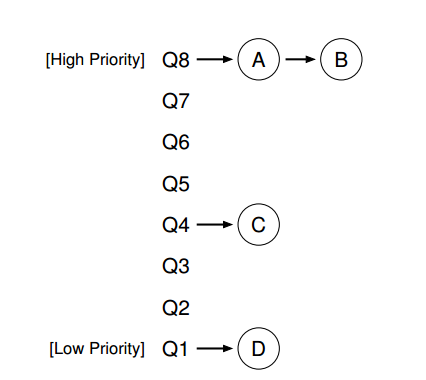
\includegraphics[width=2.4in]{1.PNG}
    \caption{The Multi-level Feedback Queue}
  \end{figure}
\end{frame}

\begin{frame}{We Need Simple Alogrithms}
  \begin{enumerate}
  \item Sometimes RTOS must guarantee events in serveral nanoseconds.       \pause
  \item Even an AND gate needs about 500 picosecond! An instruction usually needs 5ns! \pause
  \item INTEGRITY-178B uses RMA(Rate Monotonic Analysis) to reduce syscall cost.   \pause 
  \end{enumerate}
\end{frame}

\section{Problem Specification}
\begin{frame}{Periodic Hard-real-time Job Sets}              %[1]
  \begin{itemize}
  \item In this simulation, we have three or four periodic hard-real-time job sets:\\ \pause
        $S_i={J_{i1}, J_{i2}, \ldots, J_{in}}$ Each job in $S_i$ shares the same period p and the same instruction sequence length l.\pause
    \begin{itemize}
    \item $J_{ik}$ arrives at the p(k-1)-th unit of time and must be finished before the pk-th unit of time.    \pause
    \end{itemize}
  \item We need to simulate different runs under different real-time schedulers and evaluate their performance.\pause
  \end{itemize}
\end{frame}

\begin{frame}{RTOS Schedulers And Periodic Jobs}
  \begin{figure}[H]
    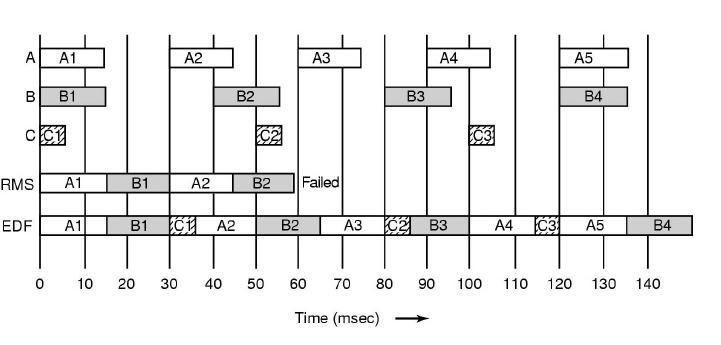
\includegraphics[width=3in]{2.PNG}
    \caption{EDF and RMS}
  \end{figure}
\end{frame}

\section{Simulation of RTOS Runtime Context}
\begin{frame}{RT OS Simulation}
  \begin{enumerate}
  \item Define tasks as sequences of instructions and a pointer to where it is executing. Each instruction costs the same constant units of time. \pause
  \item Use a paralleled thread to maintain time\_tick, continuously incrementing it. Schedulers can read it.\pause
  \item Simulate periodic job events: every p units of time, add a new job into the task list, and record the execution time of last job. \pause
  \item For simplicity, there is only one interruption in our RTOS, the clock interruption.\pause
  \item The architecture allows both preemptive and non-preemptive scheduling.\pause
  \item Global resources: tick, task list, current task pointer, PC.
  \end{enumerate}
\end{frame}

\begin{frame}{Clock Interrupt Simulation Thread}
    \lstinputlisting[label=clock,caption=clock interruption ISR simulation]{clock.c}
\end{frame}

\begin{frame}{Kernel And User Code Simulation Thread}
  \lstinputlisting[label=main,caption=main simulation thread]{user.c}
\end{frame}

\begin{frame}{Tick Updation Routine}
  \lstinputlisting[label=main,caption=main simulation thread]{time.c}
\end{frame}

\section{Analysis}
\begin{frame}{Performance Analysis}
  The analysis will include:\pause
  \begin{enumerate}
  \item The most important performance metric is the Successive Ratio and it is defined as, $SR = \frac{\text{Number of jobs successfully scheduled}}{\text{Total number of jobs arrived}}$ \pause
  \item Execution Time $E_i$.\\\pause
    $
    E_i=  
    \begin{cases}
      \mbox{execution time of the job}   &\mbox{if deadline met}\\
      0 &\mbox{if deadline not met} 
    \end{cases}
    $
  \item ECU(Effective CPU Utilization) gives information about how efficiently the processor is used and it is defined as, $ECU=\sum_{i\in R} \frac{E_i}{T}$. $T=\text{Total time of scheduling}$
  \end{enumerate}
\end{frame}


\begin{frame}
  \begin{center}
    \Huge{Q \& A}
  \end{center}
\end{frame}  



\end{document}

